\documentclass{article}
\usepackage[russian]{babel}
\usepackage[utf8]{inputenc}	
\usepackage [
	a4paper,
	left = 1 cm, 
	right = 1 cm, 
	top = 1 cm, 
	bottom = 2 cm
]{geometry}
\usepackage{wrapfig}
\usepackage[ 
	margin = 10pt, 
	font = footnotesize, 
	labelfont = bf, 
	labelsep = endash, 
	labelfont = bf, 
	textfont = rm, 
	margin = 0pt, 
	aboveskip = 4pt, 
	belowskip = -6pt
]{caption}

\usepackage[russian]{babel}
\usepackage[utf8]{inputenc}	
\usepackage{amsmath}
\usepackage{amssymb}
\usepackage{amsthm}
\usepackage{dsfont}
\usepackage{gensymb}
\usepackage{graphicx} 
\usepackage{tabularx} 
\usepackage{mathtools}
\usepackage{subcaption}
\usepackage{wrapfig}
\newcolumntype{L}[1]{>{\hsize=#1\hsize% 
\raggedright\arraybackslash}X}% 
\newcolumntype{R}[1]{>{\hsize=#1\hsize% 
\raggedleft\arraybackslash}X}% 
\newcolumntype{C}[1]{>{\hsize=#1\hsize% 
\centering\arraybackslash}X} 

\title{Домашняя работа №3}
\author{Эмиль Алкин}
\date{}
\DeclareMathOperator{\cm}{\text{см}}
\begin{document}
	\maketitle
	\section{Уран}
	\begin{wrapfigure}[12]{r}[1cm]{0.3\textwidth}
    	\centering 
    	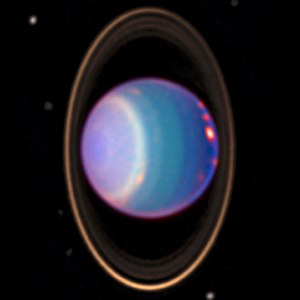
\includegraphics[width = 0.25\textwidth]{img/Uranusandrings}
    	\caption{Уран и его кольца.}
    \end{wrapfigure}  
    \hspace*{12pt} Уран~--- планета Солнечной системы, седьмая по удалённости от Солнца, третья по диаметру и четвёртая по массе. Была открыта в 1781 году английским астрономом Уильямом Гершелем и названа в честь греческого бога неба Урана.\par
    Средняя удалённость планеты от Солнца составляет $19.1914$ а. е. ($2.8$ млрд км). Период полного обращения Урана вокруг Солнца составляет $84$ земных года. Расстояние между Ураном и Землёй меняется от $2.6$ до $3.15$ миллиардов километров. Большая полуось орбиты равна $19.229$ а. е., или около $3$ миллиардов километров. Интенсивность солнечного излучения на таком расстоянии составляет $1/400$ от значения на орбите Земли.\par 
    Уран тяжелее Земли в $14.5$ раз, что делает его наименее массивной из планет--гигантов Солнечной системы. Плотность Урана, равная $1.270~\text{г}/\cm^3 $, ставит его на второе после Сатурна место среди наименее плотных планет Солнечной системы.
    \section{Спутники Урана} 
    \begin{wrapfigure}[12]{r}[1cm]{0.4\textwidth}
    	\centering 
    	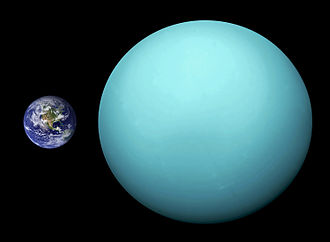
\includegraphics[width = 0.3\textwidth]{img/Uranussizecomparison}
    	\caption{Размеры Урана по сравнению с Землёй.}
    \end{wrapfigure} 
    \hspace*{12pt} В системе Урана открыто $27$ естественных спутников. Названия для них выбраны по именам персонажей произведений Уильяма Шекспира и Александра Поупа. Можно выделить пять основных самых крупных спутников: это Миранда, Ариэль, Умбриэль, Титания и Оберон.\par 
    Первые два спутника Урана, открытые в 1787~г., были названы лишь в $1852$~--- через год после обнаружения двух следующих. Их наименованием занялся Джон Гершель, сын первооткрывателя Урана. Он решил не брать названия для спутников из греческой мифологии, назвав их в честь духов из английской литературы: царя и царицы фей и эльфов Оберона и Титании из пьесы <<Сон в летнюю ночь>> Уильяма Шекспира и сильфов Ариэля и Умбриэль из <<Похищения локона>> Александра Поупа (Ариэль --- также ещё и эльф из Шекспировской <<Бури>>).\\
    \begin{center}
    \begin{tabularx}{0.5\textwidth}{|C{0.2}|C{0.6}|C{0.2}|} 
    \hline
    Номер & Название спутника & Год открытия\\ 
    \hline 
    1 & Корделия & 1986\\ 
    \hline 
    2 & Офелия & 1986\\ 
    \hline 
    3 & Бианка & 1986\\ 
    \hline 
    4 & Крессида & 1986\\ 
    \hline 
    5 & Дездемона & 1986\\ 
    \hline 
    6 & Джульетта & 1986\\ 
    \hline 
    7 & Порция & 1986\\ 
    \hline 
    8 & Розалинда & 1986\\ 
    \hline 
    9 & Купидон & 2003\\ 
    \hline 
    10 & Белинда & 1986\\ 
    \hline 
    11 & Пердита & 1986\\ 
    \hline 
    12 & Пак & 1985\\ 
    \hline 
    13 & Маб & 2003\\ 
    \hline 
    14 & Миранда & 1948\\ 
    \hline 
    15 & Ариэль & 1851\\ 
    \hline
    16 & Умбриэль & 1851\\ 
    \hline
    17 & Титания & 1787\\ 
    \hline 
    18 & Оберон & 1787\\ 
    \hline 
    19 & Франциско & 2001\\ 
    \hline 
    20 & Калибан & 1997\\ 
    \hline 
    21 & Стефано & 1999\\ 
    \hline 
    22 & Тринкуло & 2001\\ 
    \hline 
    23 & Сикоракса & 1997\\ 
    \hline
    24 & Маргарита & 2003\\ 
    \hline 
    25 & Просперо & 1999\\ 
    \hline 
    26 & Сетебос & 1999\\ 
    \hline
    27 & Фердинанд & 2001\\ 
    \hline  
    \end{tabularx}
    \end{center}
    \section{Интегрирование}
    \hspace*{12pt} Определим функцию $f(x)$:
    \begin{equation} 
    	f(x) = \begin{cases} 
    	\log_2 x, & x \geqslant 4;\\
    	\sqrt{x}, & 1 \leqslant x < 4;\\ 
    	x^2, & 0 \leqslant x < 1;\\ 
    	0, & -1 \leqslant x < 0;\\ 
    	x + 1, & x < -1. 
    	\end{cases} 
    \end{equation}\par
    Найдём производную этой функции. На интервалах $(-1, 0)$, $(0, 1)$, $(1, 4)$ производная $f(x)$ будет равна производной, соответствующей функции,
    \begin{gather} 
    f'(x)\,|_{\,(-1,\,0)} = 0' = 0,\\ 
    f'(x)\,|_{\,(0,\,1)} = (x^2)' = 2x,\\ 
    f'(x)\,|_{\,(1,\,4)} = (\sqrt x)' = \frac{1}{2\sqrt{x}}. 
    \end{gather}
    Аналогично находится производная $f(x)$ на открытых лучах $(-\infty, -1)$, $(4, +\infty)$:
    \begin{gather} 
    f'(x)\,|_{\,(-\infty,\,-1)} = (x + 1)' = 1,\\ 
    f'(x)\,|_{\,(4,\,+\infty)} = (\log_2 x)' = \frac{1}{x\ln{2} }. 
    \end{gather}
    Найдя соответствующие левые и правые производные функции $f(x)$ в точках $-1$, $0$, $1$, $4$ , можно заключить, что в этих точках производная не определена.\par
    Теперь исследуем интеграл функции $f(x)$. Пусть мы хотим найти определенный интеграл функции $f(x)$ на отрезке $[a, b]$, где $a < -1$, а $b > 4$. Тогда в силу линейности интеграла,
    \begin{multline} 
    \int\limits_{a}^{b}f(x)\,dx = \int\limits_{a}^{-1}(x+1)\,dx + \int\limits_{-1}^{0} 0\,dx + \int\limits_{0}^{1} x^2\,dx + \int\limits_{1}^{4} \sqrt x\,dx + \int\limits_{4}^{b} \log_2 x\,dx =\\ 
    = \left. \left(\frac{x^2}{2}+x\right) \right|_a^{-1} + \left. 0 \right|_{-1}^0 +\left. \left(\frac{x^3}{3}\right) \right|_0^1 + \left. \left(\frac{2\sqrt{x^3}}{3}\right) \right|_1^4 + \left. \left( x\log_2\frac{x}{e}\right) \right|_4^b = \\ 
    = 12.5 - 4\log_2 e + b\log_2 \frac{b}{e} + a - \frac{a^2}{2}. 
    \end{multline}

    \section{Затмения}
    \hspace*{12pt} Солнечное затмение~--- астрономическое явление, которое заключается в том, что Луна закрывает полностью или частично Солнце от наблюдателя на Земле.\par
    Лунное затмение~--- астраномическое явление, возникающее, когда Луна попадает в тень от Земли.\par
    \subsection*{Разновидности затмений (см. рис.\,\ref{pic:a}):}
    \begin{itemize}
    	\item Полное 
    	\item Частное
    	\item Кольцевое
    	\item Полутеневое
    \end{itemize}

    \begin{figure}[p] 
    \centering 
    \begin{subfigure}[b]{0.43\textwidth} 
    	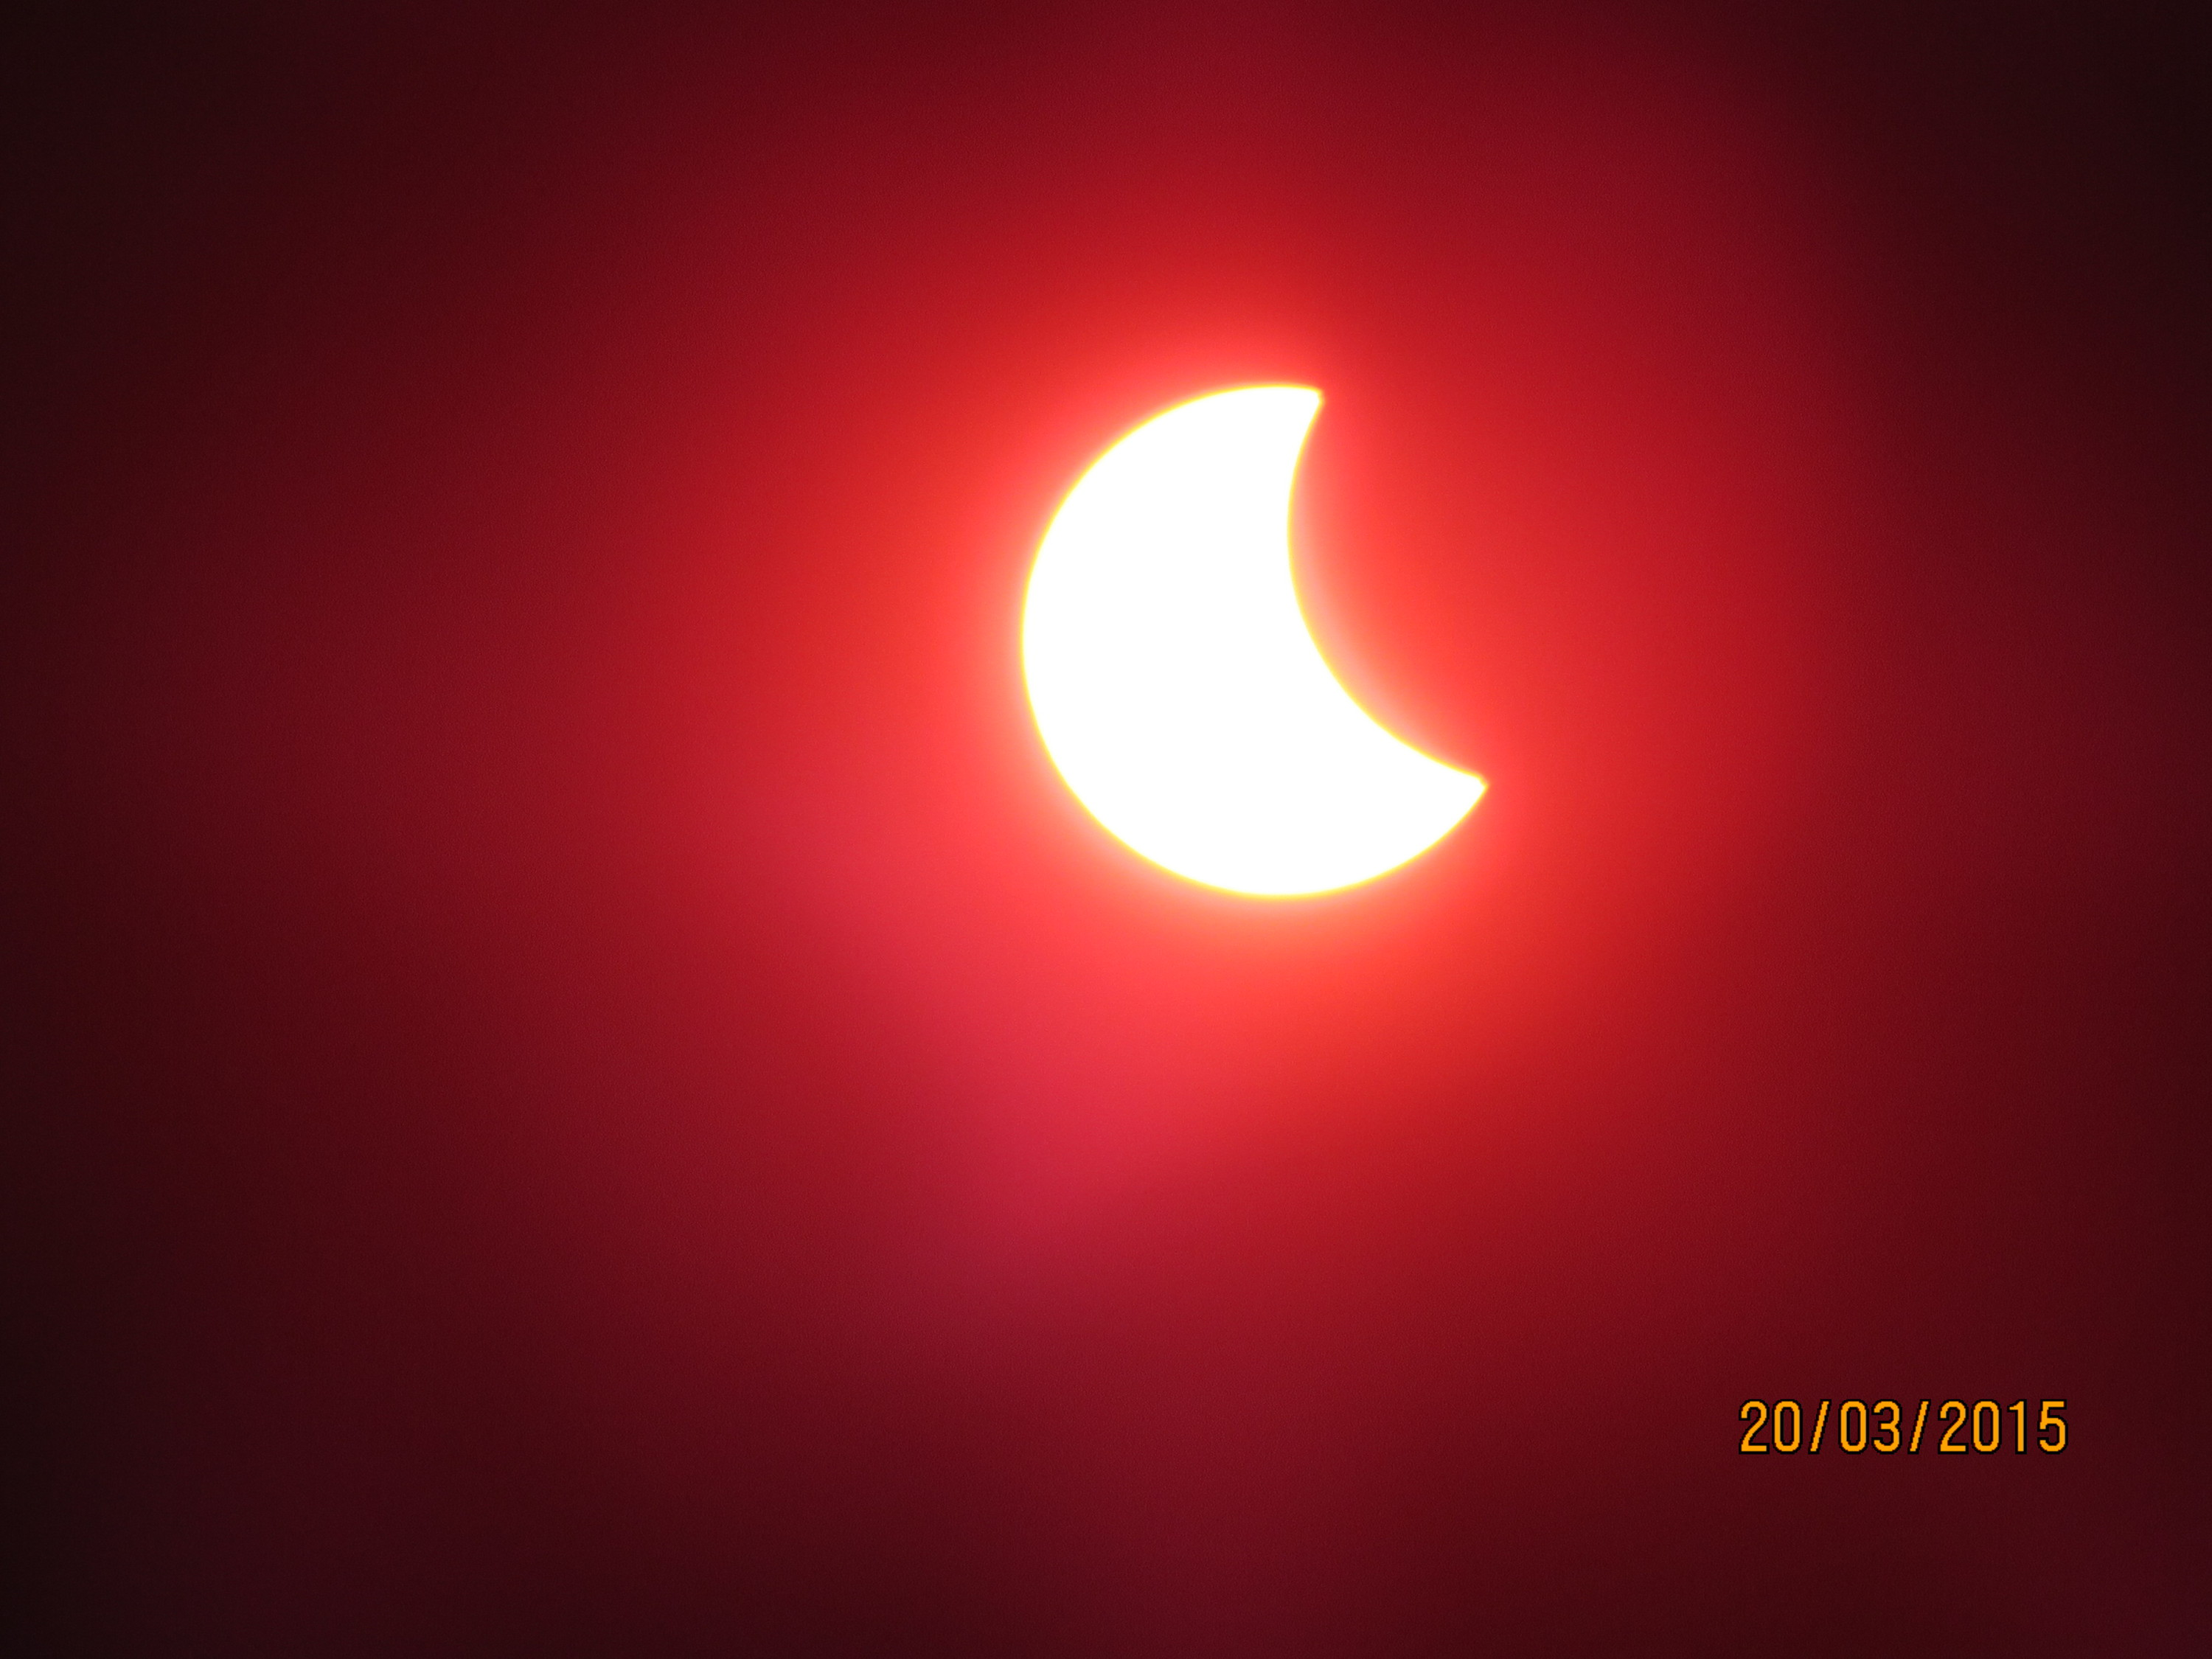
\includegraphics[width = \textwidth]{img/1} 
    	\caption{} 
    \end{subfigure} 
    \begin{subfigure}[b]{0.48\textwidth} 
    	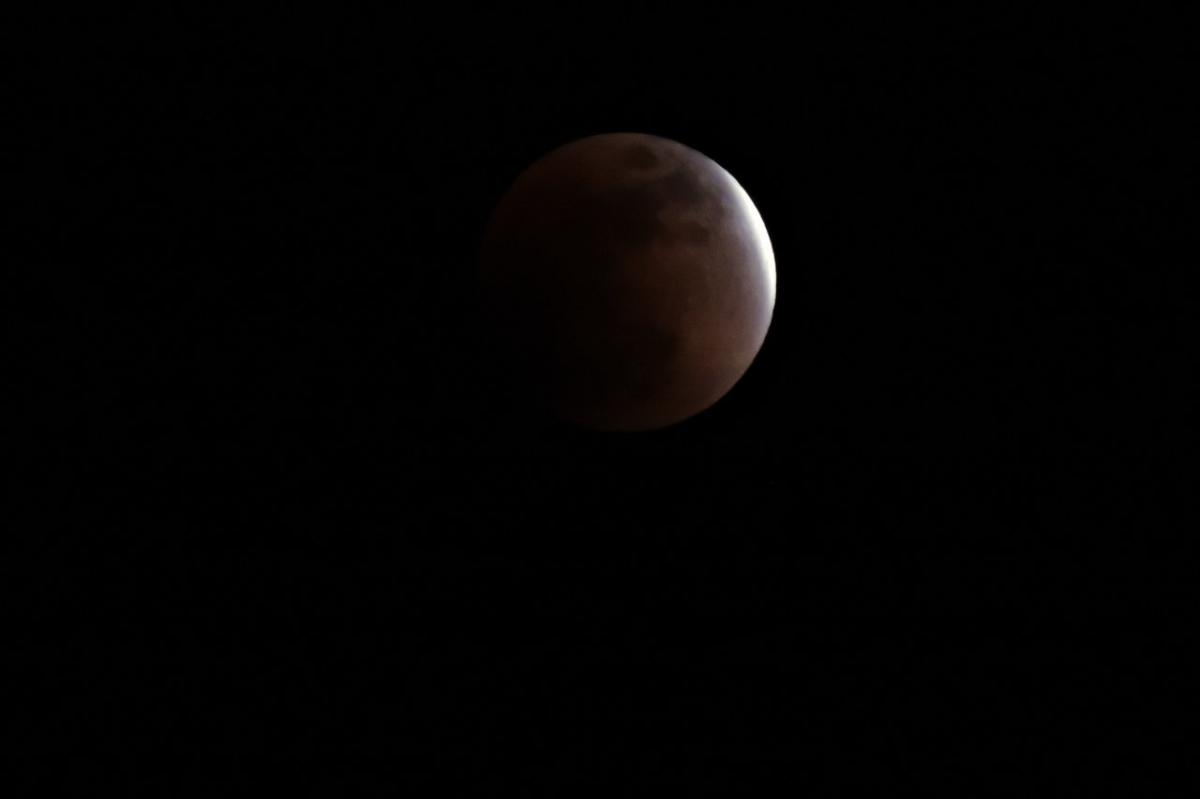
\includegraphics[width = \textwidth]{img/6} 
    	\caption{} 
    \end{subfigure} 
    \caption{Солнечное и лунное затмение} 
    \end{figure}
    
    \begin{figure}[p] 
    \centering 
    \begin{subfigure}[b]{0.45\textwidth} 
    	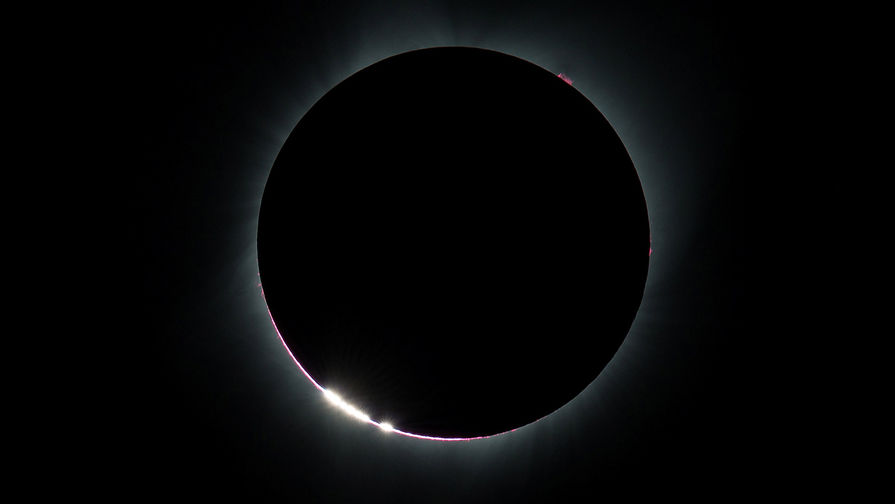
\includegraphics[width = \textwidth]{img/5}  
    	\caption{Полное затмение} 
    \end{subfigure} 
    \begin{subfigure}[b]{0.38\textwidth} 
    	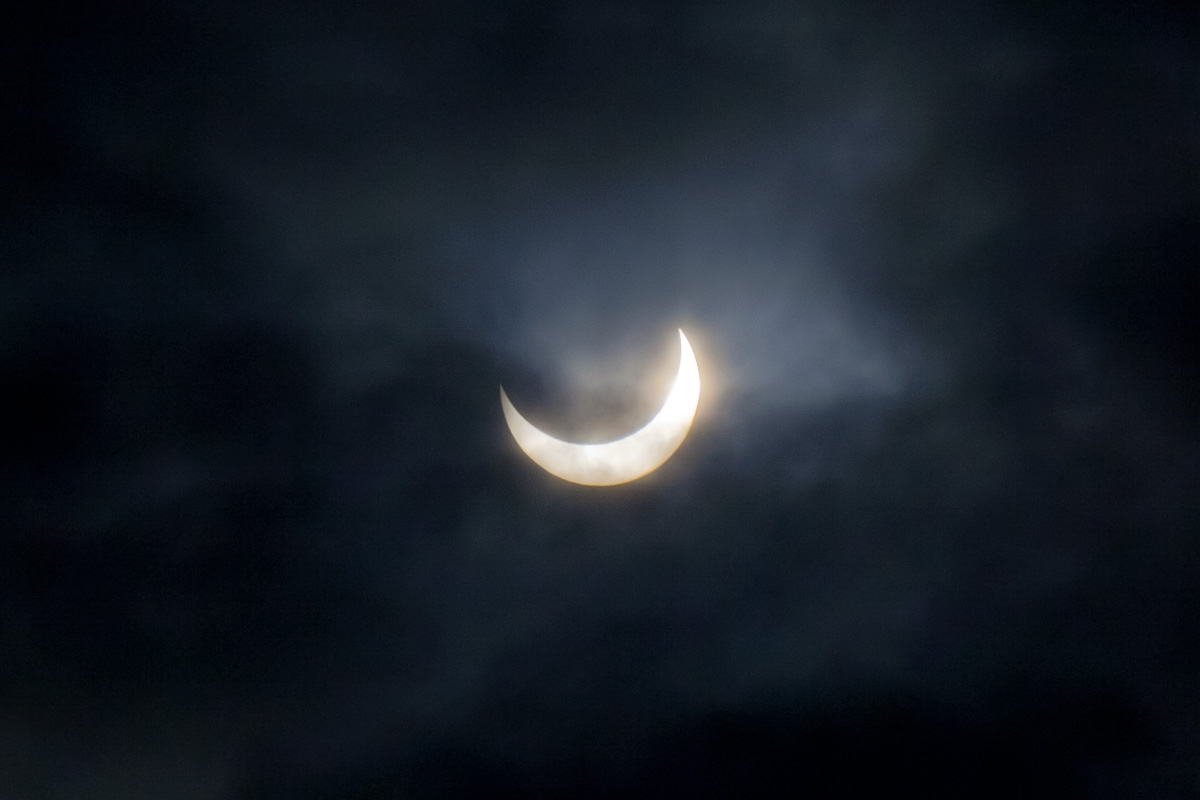
\includegraphics[width = \textwidth]{img/4} 
    	\caption{Частное затмение} 
    \end{subfigure} 
    \begin{subfigure}[b]{0.45\textwidth} 							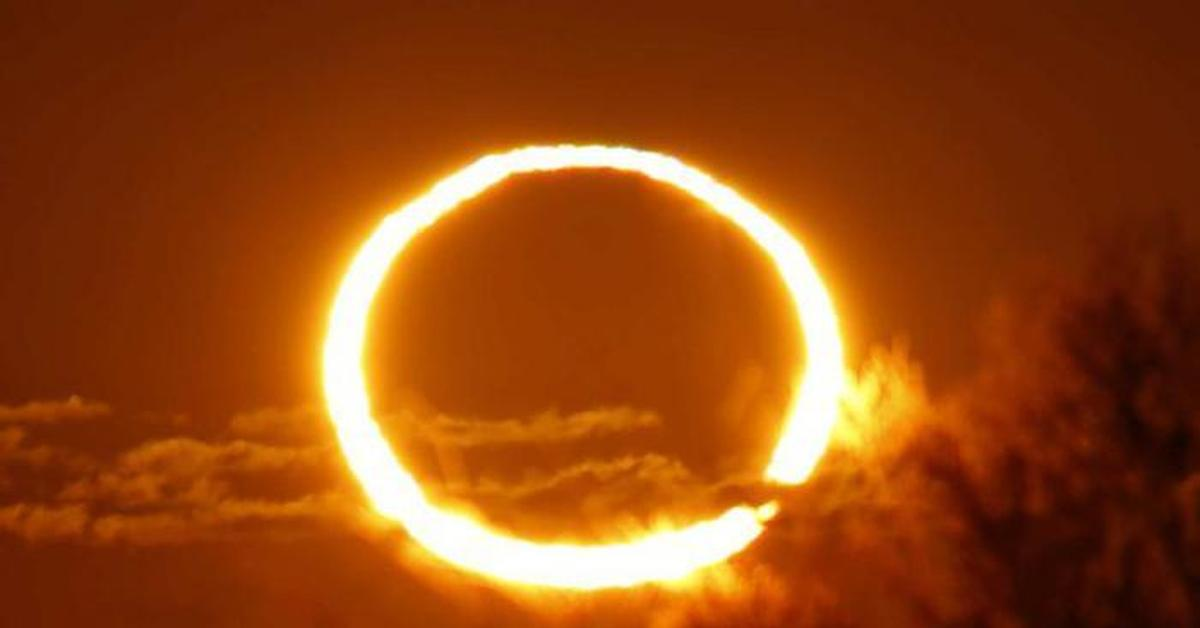
\includegraphics[width = \textwidth]{img/3} 
    	\caption{Кольцевое затмение} 
    \end{subfigure} 
    \begin{subfigure}[b]{0.29\textwidth} 							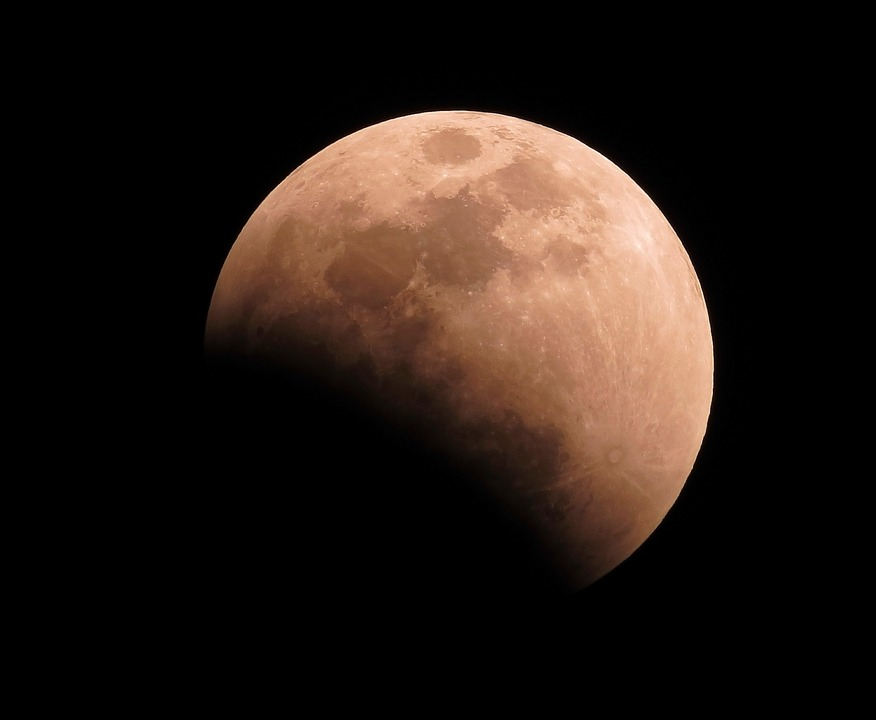
\includegraphics[width = \textwidth]{img/2} 
    	\caption{Полутеневое затмение} 
    \end{subfigure} 
    \caption{Разновидности затмений} 
    \label{pic:a}
    \end{figure}
\end{document}